\documentclass[english,11pt,a4paper]{article}

\usepackage{amsmath}
\usepackage[english]{babel}
\usepackage[utf8]{inputenc}
\usepackage{units}
\usepackage{datetime}

\usepackage[mathcal]{euscript}
\usepackage{bbm}
\usepackage{parskip}
\parskip 3mm
% \parindent 3mm

\usepackage{nicefrac}
\usepackage{wasysym}
\usepackage{enumerate}

\usepackage{graphicx}
\graphicspath{{./Graphics/}}

\usepackage{amsthm}
\newtheoremstyle{definition}
{3pt}% hSpace above
{3pt}% hSpace below
{}% hBody font
{}% hIndent amount
{\bfseries}% hTheorem head font       \itshape
{:}% hPunctuation after theorem head
{.5em}% hSpace after theorem head
{}% hTheorem head spec (can be left empty, meaning `normal')
\theoremstyle{definition}
\newtheorem{defin}{Definition}

\newtheoremstyle{remark}
{10pt}% hSpace above
{10pt}% hSpace below
{}% hBody font
{}% hIndent amount
{\bfseries}% hTheorem head font       \itshape
{:}% hPunctuation after theorem head
{.5em}% hSpace after theorem head
{}% hTheorem head spec (can be left empty, meaning `normal')
\theoremstyle{remark}
\newtheorem{remark}{Remark}

\newtheoremstyle{case}
{8pt}% hSpace above
{8pt}% hSpace below
{}% hBody font
{}% hIndent amount
{\scshape}% hTheorem head font       \itshape
{,}% hPunctuation after theorem head
{.5em}% hSpace after theorem head
{}% hTheorem head spec (can be left empty, meaning `normal')
\theoremstyle{case}
\newtheorem{case}{Case}

%\usepackage{sectsty}
%\allsectionsfont{\sffamily}
%\subsectionfont{\mdseries}


\renewcommand{\P}{\mathbf{P}}
\newcommand{\Q}{\mathbf{Q}}
\newcommand{\q}{\mathcal{Q}}
\newcommand{\J}{\mathbf{J}}
\renewcommand{\j}{\mathcal{J}}


\newcommand{\Tfi}{\widetilde T_5}
\newcommand{\Tfo}{\widetilde T_4}
\newcommand{\sumfo}{\sum_{i=1}^4 x_i}
\newcommand{\sumsumfo}{\sum_{\substack{i,j=1\\i<j}}^4 x_i x_j}

\renewcommand{\bar}{\overline}
\renewcommand{\tilde}{\widetilde}

\newcommand{\ek}{H(K)}
\newcommand{\ekb}{H(\bar K)}
\newcommand{\enk}{H_0(K)}
\newcommand{\enkb}{H_0(\bar K)}

%-------------------------------------------------------------------------%
% MASTERARBEIT (╯°□°)╯︵ ┻━┻       ┬─┬ノ( º _ ºノ)      (ノಠ益ಠ)ノ彡┻━┻   %
%-------------------------------------------------------------------------%
\begin{document} %------------   \(◕ ◡ ◕\)   -----------------------------%
% (/◔ ◡ ◔)/   ◕‿◕

\scriptsize \hfill Juri; Hyperelliptic Curves --- Draft 1.2 --- \today
\normalsize

\section{Addition Law}

\subsection{Definitions and Notation}

\begin{defin}
	Let $K$ be a field with char$(K) \neq 2$ and $\bar K$ its algebraic closure. Define the hyperelliptic curve of genus two $H_{0,C}(K)$ as the set of solutions in $K^2$ to the equation $y^2=C(x)$ where $C(x)=x^5+ax^4+bx^3+cx^2+dx+e$ is a polynomial over $K$. Write $\enk$ whenever there is no ambiguity. Similarly, the set of solutions in the closure would be denoted $\enkb$.	Define $\ek$ as $\enk \cup \{ \infty \}$.

	\textit{Note} that we could obtain a more reduced form of $C(x)$, eliminating $a$ by shifting $x$ to $(x-a/5)$. However, since this would rob us of the possibility of char$(K) = 5$ without simplifying our coming calculations in any significant manner, we refrain from using this trick.

	For the purpose of clarity, let points on the hyperelliptic curve --- in the sense of solutions to $y^2=C(x)$ --- be designated by the calligraphic letter $\q=(x,y) \in \enkb$. The point opposite to $\q$ will be written $\bar \q = (x,-y)$ and by symmetry of the curve in $y$ also belongs to $\enkb$. In the case where $\q = \infty$, define $\bar \q := \infty$. We allow ourselves to write $\pm \q$ whenever we mean in fact `either $\q$ or $\bar \q$'.

	We want to consider the set of all pairs $(\q_1,\q_2)$ and tame it with an equivalence relation with the goal of obtaining an additive group:

	Define $\J$ to be the set\scalebox{1.3}{ $\nicefrac{ \j }{\sim }$ }where $\j :=  \big\{ ( \q_1, \q_2 ) \hspace{1.5mm} \big | \hspace{1.5mm} \q_i \in \ekb \big\}$. $\J$ is called the `Jacobian' and the equivalence relation fullfills
	\begin{align*}
		(\q_1,\q_2) &\sim (\q_2,\q_1) \\
		\text{and\hspace{5mm}} (\q,\bar \q) & \sim ( \infty , \infty ). 
	\end{align*}
	Write $\{ \q_1,\q_2 \}$ from now on and let bold letters denote points on the curve in the sense of classes of unordered pairs $\P =\{ \q_1, \q_2 \} \in \J$. The point $\{ \bar \q_1, \bar \q_2 \}$ will be called $\bar \P$ for now but can already tentatively be thought of as $-\P$. Call $\{ \infty, \infty \}$ the zero of our set. We will also permit ourselves the notation $\{ \q,\bar \q \} = 0$ and we refrain from explicitly stating that $\P$ is in fact an equivalence class.

	A point $\q = (x_0,y_0)$ is called singular if it fulfills both $y_0=0$ and $C'(x_0) = 0$. A curve is called singular if and only if it has a singular point. We consider only non-singular hyperelliptics from here on.
\end{defin}


\subsection{Addition Law}

Let $\P_1 = \{\q_1,\q_2\}$, $\P_2 = \{\q_3,\q_4\}$ with $\q_i = (x_i,y_i) \in \ekb$. To define $\P_3 = \P_1 + \P_2$ we distinguish between one general case and a number of special cases and first derive the results of the former before enumerating the latter ones.

\begin{case} {\scshape Four Distinct Component-Points:}
	The overarching idea is to obtain a fifth and sixth $x$-coordinate and the corresponding $y$-coordinates by passing a polynomial of degree three through the four points $\q_i$. Ideally this should give us two additional intersections with the curve which we use as the components of our point $\P_1 + \P_2$.

	{\scshape Step 1:} Let the $\q_i$ and $\P_i$ be defined as above with $x_i \neq x_j$ whenever $i \neq j$. In addition to that, let us restrict ourselves to $\q_i \in \enk$. It is known that the Vandermonde-Matrix
	\begin{align*}V:=
		\begin{pmatrix}
			1 & x_1 & x_1^2 & x_1^3\\
			1 & x_2 & x_2^2 & x_2^3\\
			1 & x_3 & x_3^2 & x_3^3\\
			1 & x_4 & x_4^2 & x_4^3\\
		\end{pmatrix}
	\end{align*}
	has determinant $\prod_{i < j} (x_i-x_j)$ which is conveniently non-zero if and only if the $x_i$ are pairwise distinct. Let $p(x) := p_3 x^3 + p_2 x^2 + p_1 x + p_0 \in K[x]$ be the polynomial in unknown coefficients that we are looking for. With $\textbf{y} = (y_i)_{i=1}^4$ and $\textbf{p} = (p_i)_{i=0}^3$ the problem of determining $p(x)$ can be rewritten as
	\begin{align*}
		% V \cdot (p_i)_{i=0}^3 = (y_i)_{i=1}^4.
		V \cdot \mathbf{p} = \mathbf{y}
	\end{align*}
	which by invertibility of $V$ has of course a unique solution.

	{\scshape Step 2a:} Knowing the coefficients $p_i$ of $p(x)$ we first assume that $p_3 \neq 0$, so can proceed to look for the two additional solutions of the sextic equation
	\begin{align*}
		\tag{$\star$} \label{sex} C(x)-\left(p(x)\right)^2 = 0.
	\end{align*}
	Observe that this vanishes at $x_1, x_2, x_3$ and $x_4$, so write the lefthand side as $-p_3^2(x-x_1)(x-x_2)(x-x_3)(x-x_4)(x-x_5)(x-x_6)$ for $x_5$ and $x_6$ in some extension of the field $K$. Comparing the coefficients of both expressions at $x^5$ and $x^4$ yields
	\begin{align*}
		\tag{5} \sum_{i=1}^6 x_i &= \Tfi\\
		\label{four} \tag{4} \text{and\hspace{5mm}} \sum_{\substack{i,j=1\\i<j}}^6 x_i x_j &= \Tfo
	\end{align*}
	where $\Tfi = \frac{1-2 p_2 p_3}{p_3^2}$ and $\Tfo = \frac{p_2^2+2 p_1 p_3-a}{p_3^2}$
	The second expression gives
	\begin{align*}
		x_6 \sum_{i=1}^5 x_i + \sum_{\substack{i,j=1\\i<j}}^5 x_i x_j = \Tfo.
	\end{align*}
	Doing this twice and replacing $x_6$ with the information from (5) gives
	\begin{align*}
		\left(\Tfi - \sumfo - x_5\right) \left(\sumfo + x_5\right) + x_5\sumfo + \sumsumfo - \Tfo = 0.
	\end{align*}
	Replacing $\Tfi$ and $\Tfo$ with the terms
	\begin{align*}T_5 &:= \Tfi - \sumfo \\
		\text{ and\hspace{5mm}} T_4 &:= \Tfo - \sumsumfo
	\end{align*}
	one obtains the tidy quadratic equation

	\vspace{-3mm}
	\rule{\textwidth}{0.005in}
	\begin{align*}
		\tag{$\dagger$} \label{dagger} x^2 - x \cdot T_5 + \left(T_4 - T_5 \sumfo \right) = 0
	\end{align*}
	\rule{\textwidth}{0.005in}

	of which $x_5$ is one solution and --- by symmetry of the above steps --- $x_6$ the other one. Compute $y_i=p(x_i)$, $i=5,6$ to obtain $\q_5 = \{ x_5, -y_5 \}$ and $\q_6 = \{ x_6, -y_6 \}$, at which point it becomes clear that the worst-case scenario for our field extension to accomodate the new coordinates is to be quadratic. Finally we define $\P_1 + \P_2$ to be equal to $\P_3 := \{ \q_5, \q_6 \}$.

	{\scshape Step 2b:} If $p_3$ were zero, the equation \eqref{sex} would be quintic instead. We may therefore write the lefthand side as $(x-x_1)(x-x_2)(x-x_3)(x-x_4)(x-x_5)$, again for $x_5$ somewhere in $\bar K$. Comparing the coefficients at $x^4$ gives

	\vspace{-3mm}
	\rule{\textwidth}{0.005in}
	\begin{align*}
		\tag{$\dagger \dagger$} \label{dagger2} x_5 = p_2^2 - a - \sum_{i=1}^4 x_i
	\end{align*}
	\rule{\textwidth}{0.005in}

	and we may rejoice in the implication of $x_5$ staying in $K$.

	Compute $y_5 = p(x_5)$ and define $\P_1 + \P_2$ to be the point $\P_3 := \{ (x_5, y_5), \infty \}$. Since this works just as well if $p_2=0$, we are done with the general case.
\end{case}


\begin{figure}[ht]
	\rule{\textwidth}{0.005in}
	\begin{center}
		\vspace{1mm}
		% \framebox{The eight cases illustrated}
		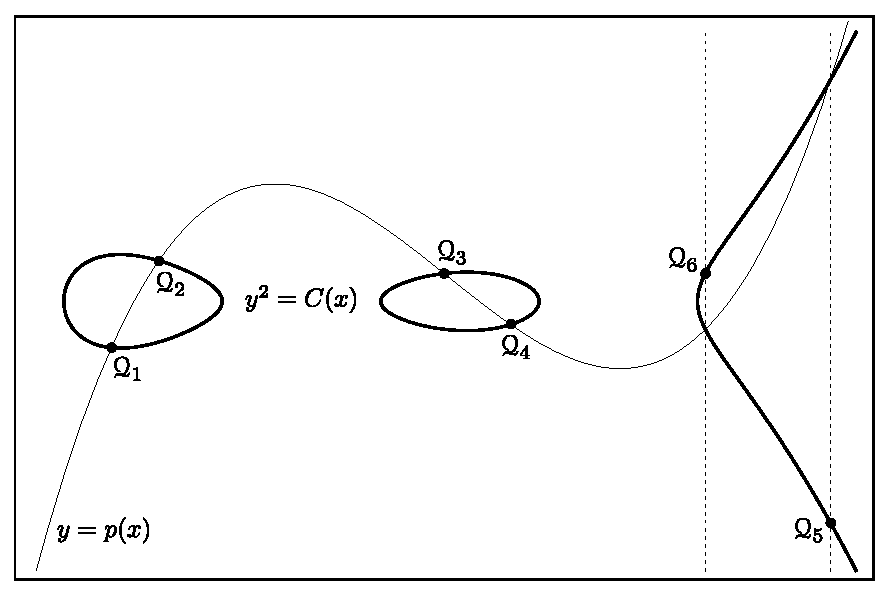
\includegraphics[width=0.9\textwidth]{addition_general.pdf}
	\end{center}
	\caption{The general case for the addition law}\label{fig_generalcase}
	\rule{\textwidth}{0.005in}
\end{figure}


Before we continue with the special cases, we want to give some consequences to the above approach.%, namely why we chose the equivalence relation the way we did for the construction of $\J$.


\textbf{Lemma:} The the general case imposes $\bar \P + \P = 0$ for all $\P \in \J$, so we might want to use the notation $\bar \P = -\P$.
\vspace{-3mm}
\begin{proof}
  (i) Observe that if $\P_1+\P_2=\P_3 \in \enkb$ as in case 1, by symmetry the polynomial $-p(x)$ passes through the opposite points, meaning that
  \begin{align*}
  	\{ (x_5,-y_5),(x_6,-y_6) \} + \{ (x_3,-y_3),(x_4,-y_4) \} = \{ (x_1,y_1),(x_2,y_2) \}
  \end{align*}
  or simply put, $\P_3+\bar \P_2=\P_1$. Since the choice of $\P_1$ and $\P_2$ was free, the statement must hold for any point $\P \in \enkb$. A similar argument can be made for the points in $\ekb$.
\end{proof}

\begin{remark}\hfill
\begin{enumerate}[(i)]
  \item The Lemma implies that if $\P+\P=0$ then $\bar \P$ equals $\P$, so the only candidates for points of order two are of the form $\{ \q, \bar \q \}$ and those that can be written as $\{ (x_1,0),(x_2,0) \}$ with $x_1 \neq x_2$, the latter being called `special points'. As defined per our equivalence relation, the special points are therefore the only non-trivial points of order two.

  \item Not only are we forced to accept the equivalence of $\{\q_1,\q_2\}$ and $\{\q_2,\q_1\}$ but if we want to construct the special cases as valid limit-cases of step 1 and 2, we must accept interchangeability between the point-components, meaning $\{\q_1,\q_2\} + \{\q_3,\q_4\}$ has to give the same result as $\{\q_1,\q_3\}+\{\q_2,\q_4\}$ and $\{\q_1,\q_4\}+\{\q_2,\q_3\}$. \ref{fig_generalcase} hints at the necessity of this property.

  \item As a bonus, this is already gives us commutativity on $\J$ for free.
\end{enumerate}
\end{remark}

\vspace{-3mm}
%another remark: we could have done it with varieties, parametrising the equation of case 1 with $t=x_2-x_1$ and transforming the equation in a really clever way to permit us to have t=0. (meaning we have the 3 vertical lines in case )

We use property (ii) to make the coming case-distinctions more concise. Since we don't care which points in $\J$ the different $\q_i$ belong to, we are allowed to impose conditions on the latter without any further specifications.

Let us first list all possible combinations that can be taken by the $x_i$ and $y_i$ provided they reside in $\bar K$:

\begin{enumerate}[A.]
	\parskip 1mm
	\item All $x_i$ are pairwise distinct.
	\item Exactly two of the $x_i$ are alike, for instance $x_1=x_2$ and
	\begin{enumerate}[a.]
		\item $y_1 = y_2 \neq 0$.
		\item $y_1 = -y_2$. \hfill $\star$
	\end{enumerate}
	\item Three x-coordinates overlap, e.g. $x_1=x_2=x_3$ and
	\begin{enumerate}[a.]
		\item All three y-coordinates are the same: $y_1 = y_2 = y_3 \neq 0$.
		\item Only two y-coordinates are alike: $y_1 = y_2$ so $y_3=-y_1$. \hfill $\star$
	\end{enumerate}
	\item All four $x_i$ are the same and
	\begin{enumerate}[a.]
		\item All four $y_i$ equal as well but non-zero.
		\item The $y_i$ overlap two by two, e.g. $y_1=y_2$ and $y_3=y_4=-y_1$. \hfill $\star$
		\item Three of the $y_i$ are alike, one isn't. \hfill $\star$
	\end{enumerate}
	\item The $x_i$ overlap two-by-two: $x_1=x_2$ and $x_3=x_4$ but $x_1 \neq x_3$ and
	\begin{enumerate}[a.]
		\item $y_1 = y_2$ plus $y_3=y_4$ but neither $y_1$ nor $y_3$ is zero.
		\item $y_1 = -y_2$, $y_3=y_4$. \hfill $\star$
		\item $y_1 = -y_2$ and $y_3=-y_4$. \hfill $\star$
	\end{enumerate}
\end{enumerate}

Due to the property that $\{ \q_i, \q_j \} \sim 0$ whenever $x_i=x_j$ and $y_i = -y_j$, every case marked with $\star$ comes down to the addition with 0. Reordering thus leads us to the following condensed list of cases for the addition law:

\vspace{-3mm}
\rule{\textwidth}{0.005in}
\begin{enumerate}\setcounter{enumi}{-1}
	\parskip 1mm
	\item The addition with zero, i.e. $\P + \{ \infty, \infty \}$ or in short $\P + 0$.
	\item The general case where all four $x$-coordinates are pairwise distinct.
	\item The simple tangential case where $\q_1 = \q_2$ and the remaining $x_3$, $x_4$ are both distinct from each other as well as from $x_1$.
	\item The double tangential case where $\q_1 = \q_2$ and $\q_3 = \q_4$ but $\q_1 \neq \pm \q_3$.
	\item Case where $\q_1=\q_2=\q_3$ but $\q_4 \neq \pm \q_1$.
	\item The quadruple case where all $\q_i$ are identical.
\end{enumerate}
\vspace{-3mm}
\rule{\textwidth}{0.005in}
\parskip 3mm

\begin{remark}\hfill
\begin{enumerate}[(i)]
	\item For the above list to be complete, we have to allow for $\q_i = \infty$ for some $i$. Note that one is sufficient, since if two or more $\q_i$ were to be $\infty$, we would be back at the zero case.

	So it is important to observe that this is already secretly included in the general case and the relevant cases 2 and 4 through the following argument:

	Suppose $\q_4 = \infty$, so the coordinate $x_4$ does not exist. The polynomial $p(x)$ we pass through the 3 remaining points is therefore necessarily at most quadratic instead of cubic so the corresponding matrix to invert is the upper left 3x3 sub-matrix of $V$, $V'$ or $V'''$. We are then immediately sent to \eqref{dagger2} of the second step.

	\item In both lists, the cases do not overlap.
\end{enumerate}
\end{remark}

% \begin{figure}[!ht]
% 	\rule{\textwidth}{0.005in}
% 	\begin{center}
% 		\vspace{3mm}
% 		% \framebox{The eight cases illustrated}
% 		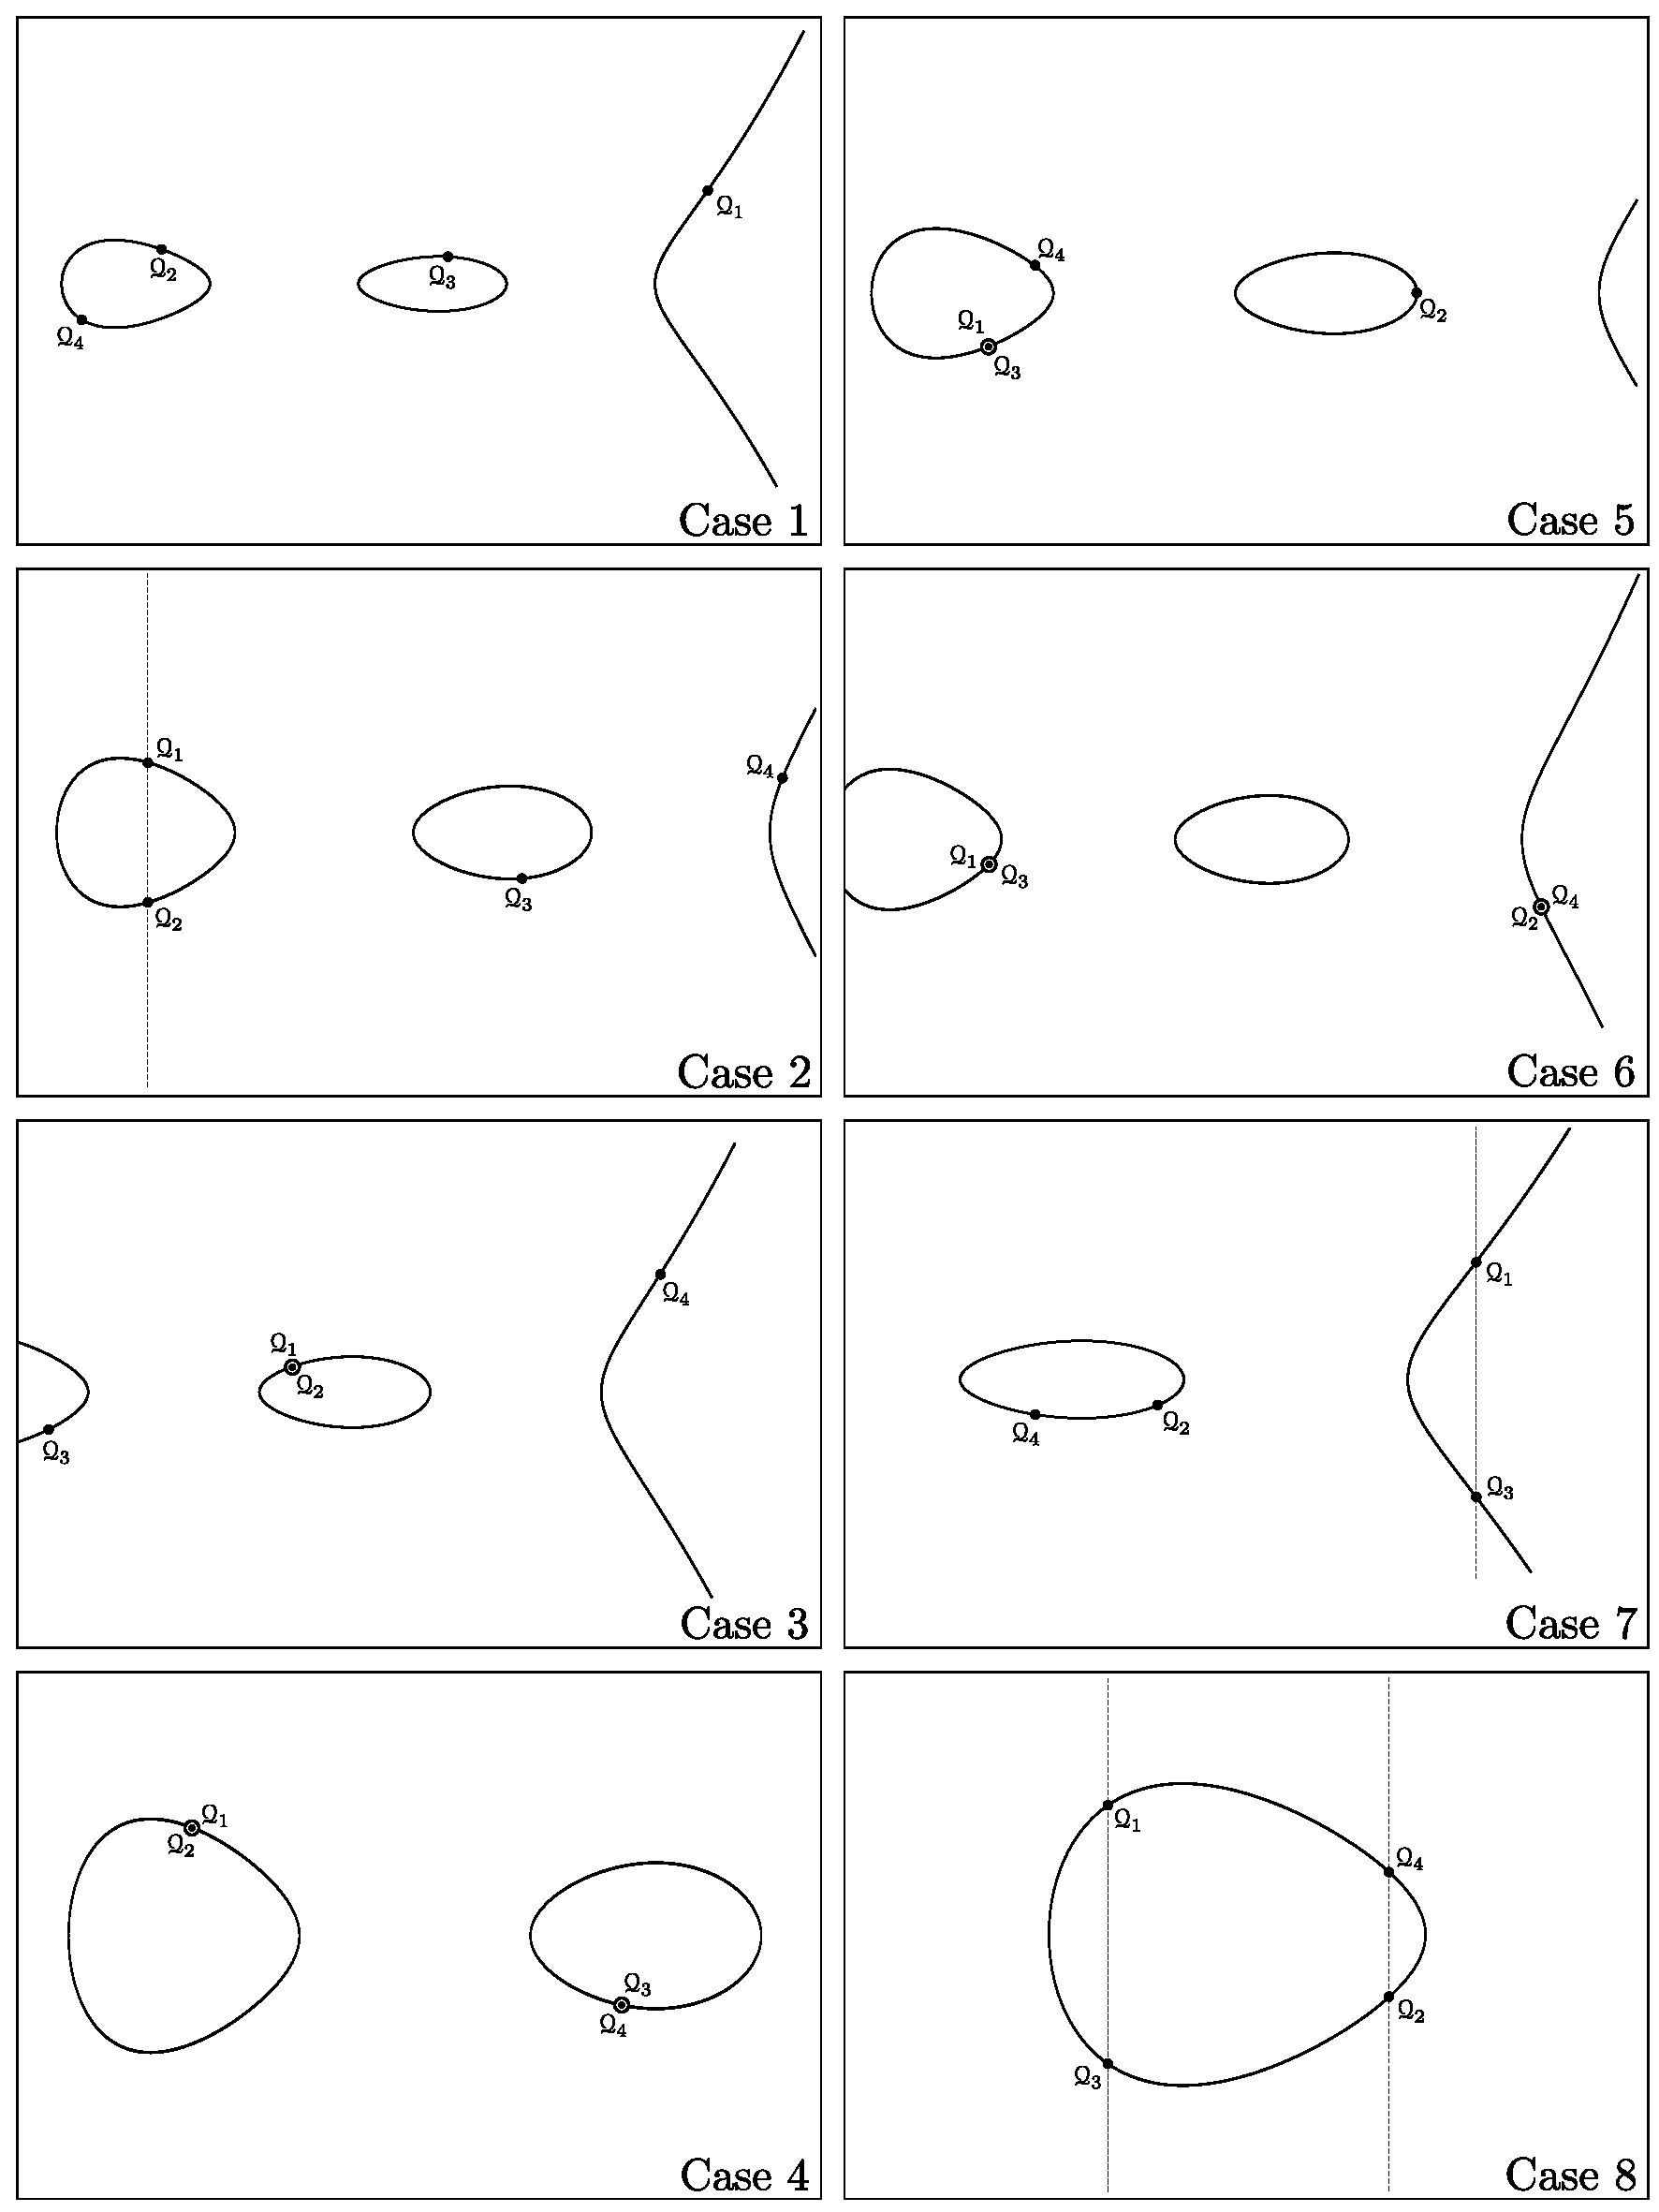
\includegraphics[width=0.9\textwidth]{addition_laws_all.pdf}
% 	\end{center}
% 	\caption{Examples for all 8 possible configurations of points in $\mathbbm R^2$.}\label{fig_eightcases}
% 	\rule{\textwidth}{0.005in}
% \end{figure}

\setcounter{case}{-1}

\begin{case}
  {\scshape Addition with Zero:} As one might have anticipated, if $\P_2 = 0$ we define $\P_1 + \P_2 = \P_1$ for every $\P_1 \in \J$.
\end{case}

\setcounter{case}{1}
\begin{case}
	{\scshape Tangential:} Let $\q_1 = \q_2$, $y_1 \neq 0$ but $x_1$, $x_3$ and $x_4$ are pairwise distinct. We cannot use the Vandermonde Matrix in this case because it won't possess maximal rank, consequently being non-invertible. We can however obtain an additional equation by demanding that our polynomial $p(x)$ be tangential to the curve at $\q_1$. This gives
	\begin{align*}
	  2 y \frac{dy}{dx} &= 5  x^4 + 4 a x^3 + 3 b x^2 + 2 c x + d \\
	  \text{and\hspace{8mm}} \frac{dy}{dx} &= 3 p_3 x^2 + 2 p_2 x + p_1
	\end{align*}
	meaning that the system to solve for $\mathbf{p}$ is now $V' \cdot \mathbf{p} = \mathbf{y'}$ with
	\begin{align*}V':=
		\begin{pmatrix}
			1 & x_1 & x_1^2 & x_1^3\\
			0 & 1 & 2 x_1 & 3 x_1^2\\
			1 & x_3 & x_3^2 & x_3^3\\
			1 & x_4 & x_4^2 & x_4^3\\
		\end{pmatrix}
	\end{align*}
	and $\mathbf{y'}$ defined as $\mathbf{y}$ with $y_2$ replaced by $y_2':=\frac{C'(x_1)}{2 y_1}$ which is well defined since $2y_1 \neq 0$.

	One can see that $V'$ is invertible by substracting $x_1$ times the previous column from every column and using Laplace:
	\begin{align*}\det (V') &=
		\begin{vmatrix}
			1 & 0 & 0 & 0\\
			0 & 1 & x_1 & x_1^2\\
			1 & (x_3-x_1) & x_3(x_3-x_1) & x_3^2(x_3-x_1)\\
			1 & (x_4-x_1) & x_4(x_4-x_1) & x_4^2(x_4-x_1)\\
		\end{vmatrix}
		\\
		&= (x_3-x_1)(x_4-x_1)
		\begin{vmatrix}
			1 & x_1 & x_1^2\\
			1 & x_3 & x_3^2\\
			1 & x_4 & x_4^2\\
		\end{vmatrix}.
	\end{align*}

	Fitting perfectly well with our constraints, this expression is non-zero exactly in the case where $x_1, x_3$ and $x_4$ are pairwise distinct.

	Once $p(x)$ is determined, step two will be entirely identical to the general case and we can again solve \eqref{dagger2} or \eqref{dagger} for $x_5$ or $x_5$ and $x_6$.

\end{case}

\begin{case}
	{\scshape Double Tangential:} Let $\q_1 = \q_2$ and $\q_3 = \q_4$ but $x_1 \neq x_3$ and $\q_i \neq \pm \q_i$ meaning that neither $y_1$ nor $y_3$ will be zero. Like before, we lack equations for our linear system, requiring the use of a second tangential constraint. Replace the fourth row of $V'$ and $\mathbf{y'}$ exactly like we did for the second one: $y_4'':=\frac{C'(x_3)}{2 y_3}$ and
	\begin{align*}V''=
		\begin{pmatrix}
			1 & x_1 & x_1^2 & x_1^3\\
			0 & 1 & 2 x_1 & 3 x_1^2\\
			1 & x_3 & x_3^2 & x_3^3\\
			0 & 1 & 2 x_3 & 3 x_3^2\\
		\end{pmatrix}.
	\end{align*}

	$V''$ is invertible by a similar transformation to that of the previous case:
		\begin{align*}\det (V'') &= 
		\begin{vmatrix}
			1 & 0 & 0 & 0\\
			0 & 1 & x_1 & x_1^2\\
			1 & (x_3-x_1) & x_3(x_3-x_1) & x_3^2(x_3-x_1)\\
			0 & 1 & 2x_3 - x_1 & 3x_3^2-2x_1x_3\\
		\end{vmatrix}
		\\
		&= (x_3-x_1)
		\begin{vmatrix}
			1 & x_1 & x_1^2\\
			1 & x_3 & x_3^2\\
			1 & (2x_3 - x_1) & (3x_3^2-2x_1x_3)\\
		\end{vmatrix}
		\\
		&= (x_3-x_1)
		\begin{vmatrix}
			1 & x_1 & x_1^2\\
			1 & x_3 & x_3^2\\
			-1 & - x_1 & x_3^2-2x_1 x_3\\
		\end{vmatrix}
		\\		
		&= (x_3-x_1)
		\begin{vmatrix}
			1 & x_1 & x_1^2\\
			0 & x_3-x_1 & x_3^2-x_1^2\\
			0 & 0 & -(x_3-x_1)^2\\
		\end{vmatrix}.
	\end{align*}

	This is again different from zero precisely whenever $x_3 \neq x_1$, so as before solve $V'' \cdot \mathbf{p} = \mathbf{y''}$ for $\mathbf{p}$, then \eqref{dagger} or \eqref{dagger2} depending on $p_3$.
\end{case}

\begin{case}
	{\scshape Second Order Tangential:} Let $\q_1=\q_2=\q_3$ but $x_1 \neq x_4$ and $y_1 \neq 0$. We can thus see this as a third-order intersection and demand that the curve and the polynomial share a second-order derivative at $\q_1$:
	\begin{align*}V'''=
			\begin{pmatrix}
			1 & x_1 & x_1^2 & x_1^3\\
			0 & 1 & 2 x_1 & 3 x_1^2\\
			0 & 0 & 2 & 6x_1\\
			1 & x_4 & x_4^2 & x_4^3\\
		\end{pmatrix}.
	\end{align*}	
	This is invertible in the given circumstance because
	\begin{align*}\det (V''') &=
		\begin{vmatrix}
			1 & 0 & 0 & 0\\
			0 & 1 & x_1 & x_1^2\\
			0 & 0 & 2 & 4x_1\\
			1 & x_4-x_1 & x_4(x_4-x_1) & x_4^2(x_4-x_1)\\
		\end{vmatrix}
		\\
		&= 2 (x_4-x_1)
		\begin{vmatrix}
			1 & x_1 & x_1^2\\
			0 & 1 & 2x_1\\
			1 & x_4 & x_4^2\\
		\end{vmatrix}
		\\
		&= 2 (x_4-x_1)
		\begin{vmatrix}
			1 & 0 & 0\\
			0 & 1 & x_1\\
			1 & x_4-x_1 & x_4(x_4-x_1)\\
		\end{vmatrix}
		\\
		&= 2 (x_4-x_1)^3 \neq 0 \text{ for } x_1\neq x_4.
	\end{align*}
	With this, define $\mathbf{y'''}$ by taking $\mathbf{y'}$ and replacing the third coordinate by $y_3''' := \frac{C''(x_1)}{2y_1}-(\frac{C'(x_1)}{2y_1})^2$. Again, apply the same procedure as in the second steps of case 1 to find $\P_3$.
\end{case}

\begin{case}
	{\scshape Third Order Tangential:} Given the quadruple situation where $\q_i = \q$ for every $i$ and knowing the point $\q := (x_0,y_0)$ with $y_0 \neq 0$, we solve
	\begin{align*}V'''' &=
		\begin{pmatrix}
			1 & x_0 & x_0^2 & x_0^3\\
			0 & 1 & 2 x_0 & 3 x_0^2\\
			0 & 0 & 2 & 6x_0\\
			0 & 0 & 0 & 6\\
		\end{pmatrix}
	\end{align*}
	which is invertible in all fields but those of characteristic 2 and 3.

	Here $\mathbf{y}''''$ is the same as $\mathbf{y}'''$ except for the last coordinate which should read
	\begin{align*}
		y_4''' := \frac{1}{2y_0}\Big( C'''(x_0) - \frac{dy}{dx}\bigg|_{\q}\Big(\big(\frac{dy}{dx}\bigg|_{\q}\big)^2 - \frac{d^2y}{dx^2}\bigg|_{\q} \Big) \Big).
	\end{align*}
	The derivatives are known through the previous steps. Once more, we solve the linear system $V'''' \cdot \mathbf{p}=\mathbf{y''''}$ and subsequently \eqref{dagger} or \eqref{dagger2} and we're done.
\end{case}



% -----------------------------------------------------------------------------
% THIS IS THE END. MY ONLY FRIEND, THE END. OF EVERYTHING THAT STANDS, THE END.
% NO SADNESS NOR SURPRISE, THE END.
% CAN YOU PICTURE WHAT WILL BE? SO LIMITLESS AND FREE.
% -----------------------------------------------------------------------------
\end{document}